%\documentclass[12pt]{article}
%\usepackage[a4paper, margin=1in]{geometry} 
%\usepackage{graphicx} 
%\usepackage{hyperref}
%\usepackage{float}
%\usepackage{multicol}
%\usepackage{amsmath}
%\usepackage[font=small, labelfont=bf]{caption}
%
%\begin{document}

%
% Affine gap penalties with a single DP table
%
\subsection{Affine gap penalties with a single DP table}

%
% DP for general gap penalty
%
\subsubsection*{DP for general gap penalty}
We need to modify DP so that extra cells are checked to find the optimal score of a cell. 

%
% Cell update rule of general gap penalty
%
\subsubsection*{Cell update rule of general gap penalty}
\null \medskip  
\begin{equation*}
H_{i,j} =\max \left[H_{i-1,j-1} + R_{q_{i}d_{j}}, \quad \max_{1 \leq l \leq j}(H_{i,j-l} - g_l) ,  \quad \max_{1 \leq l \leq i}(H_{i-l,j} - g_l) \right]
\end{equation*}

%
% NEWPAGE
%
\newpage

\noindent
\textbf{Example of cell update}

\begin{multicols}{2}
Sequences:
\begin{verbatim}
    q: AG, d: ACG
\end{verbatim}
\vfill\null
\columnbreak

\noindent
Scoring scheme: \\
\null \quad $g_{open}$ = 1 \\
\null \quad $g_{extend}$ = 0.1 \\
\null \quad $R_{ab}$ = 1 for a = b \\ 
\null \quad $R_{ab}$ = 0 for a $\neq$ b \\ 

\end{multicols} 

\textbf{Update $H_{2,1}$}

\begin{figure}[H]
  \centering
      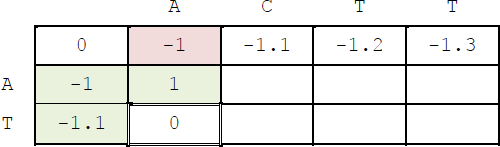
\includegraphics[width=0.5\textwidth]{fig03/dp_general_gap_example_1.png}
\end{figure}

\begin{itemize}
\item vertical:   $max(1 - 1, \quad -1 - 1 - 0.1) = 0$
\item horizontal: $-1.1 - 1 = -2.1$
\item diagonal: $-1 - 0 = -1$
\end{itemize}

\null \medskip 
\textbf{Update $H_{1,2}$}

\begin{figure}[H]
  \centering
      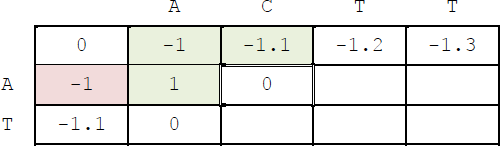
\includegraphics[width=0.5\textwidth]{fig03/dp_general_gap_example_2.png}
\end{figure}

\begin{itemize}
\item vertical: $-1.1 - 1 = -2.1$
\item horizontal: $max(1 - 1, \quad -1 - 1 - 0.1) = 0$
\item diagonal: $-1 - 0 = -1$
\end{itemize}

\null \medskip 
\textbf{Update $H_{1,3}$}

\begin{figure}[H]
  \centering
      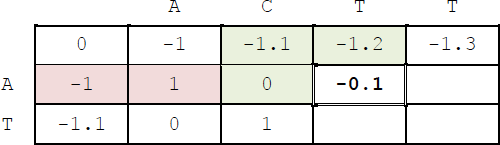
\includegraphics[width=0.5\textwidth]{fig03/dp_general_gap_example_3.png}
\end{figure}

\begin{itemize}
\item vertical: $-1.2 - 1 = -2.2$
\item horizontal: $max(0 - 1, \quad 1 - 1 - 0.1, \quad  -1 -1 - 0.1 - 0.1) = -0.1$
\item diagonal: $-1.1 - 0 = -1.1$
\end{itemize}


%
% Exercise \thesection.3
%
\subsubsection*{Exercise \thesection.3}
Complete the DP table below.

\begin{multicols}{2}
Sequences:
\begin{verbatim}
    q: AT, d: ACTT
\end{verbatim}
\vfill\null
\columnbreak

\noindent
Scoring scheme: \\
\null \quad $g_{open}$ = 1 \\
\null \quad $g_{extend}$ = 0.1 \\
\null \quad $R_{ab}$ = 1 for a = b \\ 
\null \quad $R_{ab}$ = 0 for a $\neq$ b \\ 

\end{multicols} 

\begin{figure}[H]
  \centering
      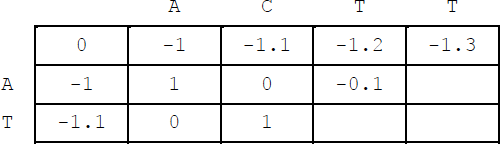
\includegraphics[width=0.5\textwidth]{fig03/dp_general_gap_exercise.png}
\end{figure}

%\end{document}
